\documentclass{article}
\usepackage[hmargin=1.25in, vmargin=.75in]{geometry}
\usepackage{amsmath, amssymb}
\PassOptionsToPackage{quiet}{fontspec}
\usepackage{ctex}
\usepackage{graphicx}
\usepackage{fancyhdr}
\pagestyle{fancy}
\def\headrule{}
\setlength{\headheight}{5em}
\fancyhead[L]{
\includegraphics[width=8em]{Logos.pdf}\large\bfseries\color{Cyan} 学习数学\ 领悟数学\ 秒杀数学}
\fancyhead[R]{\large\bfseries\color{Cyan} 第一章\ \ 三角函数}
\fancyfoot[C]{\thepage}
\usepackage{kantlipsum}
\setlength{\parindent}{0pt}
\usepackage{xcolor}
\definecolor{Cyan}{HTML}{00B0EF}
\definecolor{lightCyan}{HTML}{DDEAF5}
\hbadness20000
\usepackage{ztikz}
\ztikzLoadModule{cache, gnuplot}
\usetikzlibrary{arrows.meta}

% choices Env
\newcounter{choice}
\setcounter{choice}{1}
\newcommand\choicePunct{.\;}
\NewDocumentEnvironment{choices}{}{
  \begin{center}
}{\hfill\end{center}\setcounter{choice}{1}}
\NewDocumentCommand{\choice}{sO{\hfill}}{
  \ifnum\thechoice=1\else#2\fi%
  \IfBooleanTF{#1}{\underline{\Alph{choice}}}{\Alph{choice}}%
  \choicePunct\stepcounter{choice}%
}


% example Env
\newcounter{example}
\setcounter{example}{1}
\NewDocumentEnvironment{example}{}{
  \textcolor{Cyan}{【例\ \theexample】}
}{\stepcounter{example}}

% solution env
\newbox\solutionbox
\newlength{\solutionBoxHt}
\NewDocumentEnvironment{solution}{+b}{
  \colorBack{\textcolor{Cyan}{【解】}#1}
}{}
\NewDocumentCommand{\colorBack}{O{lightCyan}+m}{
  \setbox\solutionbox\vbox{#2}%
  \textcolor{#1}{\rule[-\dp\solutionbox]{\linewidth}{\dimeval{\ht\solutionbox+\dp\solutionbox}}}%
  \hskip-\linewidth\copy\solutionbox
}


\begin{document}
\everymath{\displaystyle}
\begin{example}
  函数 $y=2\sin(3x+\frac{\pi}{6}), x\in \mathbb{R}$ 的最小正周期是(\ ) 
  \begin{choices}
    \choice $2\pi$
    \choice* $\pi$
    \choice $\frac{2\pi}{3}$
    \choice $\frac{\pi}{3}$
  \end{choices}
\end{example}

\begin{solution}
  $T=\frac{2\pi}{\omega} = \frac{2\pi}{3}$, 故选 B.
\end{solution}


\begin{example}
已知 $y=A\sin(\omega x + \frac{\pi}{4})\; (\omega>0)$ 的最小正周期为 $\pi$, 则函数 $f(x)$ 的图像(\ )
\begin{choices}
  \choice 关于直线 $x=\frac{\pi}{4}$ 对称 
  \choice* 关于直线 $x=\frac{\pi}{8}$ 对称
  \choice[\\] 关于点 $(\frac{\pi}{4}, 0)$ 对称
  \choice 关于点 $(\frac{\pi}{8}, 0)$ 对称
\end{choices}
\end{example}


\begin{solution}
由函数 $y=A\sin(\omega x + \frac{\pi}{4})$ 的最小正周期为 $\pi$, 可得 $T = \frac{2\pi}{\omega}=\pi$, 求得 $\omega=2$,
$y=A\sin(2x+\frac{\pi}{3})$. 由于当 $x=\frac{2k\pi + \frac\pi2-\varphi}{\omega}=k\pi + \frac\pi8$ 时,函数 $f(x)$ 取得最大值为 1,
故函数 $f(x)$ 的图像关于直线 $x=\frac{\pi}{8}$ 对称, 故选 B. 
\end{solution}


\begin{example}
设函数 $f(x) = A\sin(\omega x + \varphi)\; (A\neq 0, \omega>0, -\frac{\pi}{2}<\varphi<\frac\pi2)$ 的图像关于直线 $x=\frac{2\pi}{3}$
对称, 它的最小正周期为 $\pi$, 则 (\ )
\begin{choices}
  \choice $f(x)$ 的图像过点 $(0, \frac12)$
  \choice $f(x)$ 在 $\left[\frac\pi{12},\frac{2\pi}{3}\right]$ 上是减函数
  \choice*[\\] $f(x)$ 的一个对称中心为 $(\frac{5\pi}{12}, 0)$
  \choice $f(x)$ 的一个对称中心为 $(\frac{\pi}{6}, 0)$
\end{choices}
\end{example}

\begin{solution}
由题意可得 $T=\frac{2\pi}{\omega} = \pi$, 所以 $\omega=2$, 可得 $y=A\sin(\omega x+ \varphi)$. 再由函数关于
$x=\frac{2\pi}{3}$ 对称,故 $\frac{2\pi}{3} = \frac{k\pi + \frac\pi2 -\varphi}{\omega} = \frac{k\pi + \frac\pi2-\varphi}{2}
\Rightarrow \varphi=k\pi + \frac\pi6$, 取 $\varphi=\frac\pi6$,故函数 $f(x) = A\sin(2x+\frac\pi6)$. 函数图像如下:

\begin{center}
  \begin{tikzpicture}[>=Latex]
    \xAxis[-5.5][5.5]
    \yAxis[-2.5][2.5]
    % \draw[->] (-5.5, 0) -- (5.5, 0);
    % \draw[->] (0, -2.5) -- (0, 2.5);
    \Plot[-pi:pi][Cyan, thick]{2*sin(2*x+pi/6)}
  \end{tikzpicture}
\end{center}

根据公式 $\left[\frac{2k\pi + \frac\pi2 -\phi}{\omega}, \frac{2k\pi + \frac{3\pi}2 -\phi}{\omega}\right]$ 可求得函数的减区间为
$[k\pi+\frac\pi6, k\pi+\frac{2\pi}3]$, B 错. 由于 A 不确定, 故选项 A 不正确. 对称中心为 $(\frac{k\pi-\phi}{\omega}, 0)$, 
即 $(\frac{k\pi}{2}-\frac{\pi}{12}, 0)$, $k=1$ 时,选项 C 正确. 选项 D 不正确.
\end{solution}



\end{document}







\documentclass{article}
\usepackage[T1]{fontenc}


\begin{document}
\ExplSyntaxOn
\tl_set:Nn \l_tmpa_tl {a}
\tl_set:Nn \l_tmpb_tl {b}

\tl_new:N \l_tmpc_tl
\tl_new:N \l_tmpd_tl
% \tl_set:Nn \l_tmpc_tl {\l_tmpa_tl}
% \tl_set:Ne \l_tmpd_tl {\l_tmpa_tl \exp_not:N\l_tmpb_tl}
% \cs_meaning:N \l_tmpc_tl\par
% \cs_meaning:N \l_tmpd_tl\par


% \tl_set:Nn \l_tmpa_tl {a\l_tmpb_tl}
% \tl_set:Nn \l_tmpb_tl {b}
% \tl_set:Nx \l_tmpd_tl {\l_tmpb_tl \tl_tail:N\l_tmpa_tl}
% \cs_meaning:N \l_tmpd_tl\par


% ==> protect comamnd
\tl_set:Nn \l_tmpa_tl {a}
\protected\def\cmda{CMD-A}
\newcommand\cmdb{CMD-B}
\NewDocumentCommand\cmdc{}{CMD-C}
\tl_set:Nx \l_tmpb_tl {\l_tmpa_tl \cmda \noexpand\cmdb \cmdc}
\cs_meaning:N \l_tmpb_tl\par
\tl_set:Nn \l_tmpb_tl {}


% ==> robust command
\tl_set:Nn \l_tmpa_tl {a}
\DeclareRobustCommand\robcmd{ROBUST-CMD}
\tl_set:Nx \l_tmpb_tl {\l_tmpa_tl \robcmd}
\cs_meaning:N \l_tmpb_tl\par
\tl_set:Nn \l_tmpb_tl {}


% ==> expandable command
\tl_set:Nn \l_tmpa_tl {a}
\newcommand{\expandcmd}{EXPAND-CMD}
\tl_set:Nx \l_tmpb_tl {\l_tmpa_tl \expanded{\expandcmd}}
\cs_meaning:N \l_tmpb_tl\par


% \cs_cs_generate_variant:Nn \tl_set:Nn {Nx}
% \tl_set:Nx \l_tmpc_tl {\l_tmpa_tl}
\cs_new:Nn \example:n {
  \tl_map_inline:nn { 1 2 3 } {#1}
}
\cs_generate_variant:Nn \example:n { x, e }
\ExplSyntaxOff


\def\aaa{aaa}
\def\Oldupercase#1{
  \uppercase{#1}
}
\def\Newupercase#1{
  \expanded{\uppercase{#1}}
}
\Oldupercase{\aaa}\Newupercase{\aaa}
\end{document}




\documentclass{article}
\usepackage{amsmath}
\usepackage[a3paper, margin=1in]{geometry}



\ExplSyntaxOn
\int_new:N \g_depth_int
\int_gset:Nn \g_depth_int {0}
\seq_new:N \g_data_collect_seq
\prg_generate_conditional_variant:Nnn \int_compare:nNnT {eNn}{T}

% ==> ONE-ARGUMENT RECURSION
\newcommand{\INT}[1]{
  \int_compare:nNnTF {\g_depth_int} < {5}{
    \int_gadd:Nn \g_depth_int {1}
    \seq_gput_right:Nn \g_data_collect_seq {#1}
    % \INT{[-#1-)}
    % \INT{\int^{#1}} 
    % \INT{\int\c_math_subscript_token{#1}}
  }{
    % #1
    % \seq_use:Nn \g_data_collect_seq {\par}
    \seq_item:Nn \g_data_collect_seq {-1}
    \seq_item:Nn \g_data_collect_seq {-2}
    % \par RECURSION-DEPTH:\int_use:N \g_depth_int
  }
}


% ==> TWO-ARGUMENT RECURSION
\seq_new:N \g_data_collect_I_seq
\seq_new:N \g_data_collect_II_seq
% ARGUMENTS SPECIFICATION
% #1 -> subscript
% #2 -> superscript
% #3 -> total depth
% split tree using the '\int_case:nn'
\newcommand\NEWINT[3]{
  \int_compare:nTF {\g_depth_int <= #3}{
    \int_gadd:Nn \g_depth_int {1}
    \seq_gput_right:Nn \g_data_collect_I_seq {#1}
    \seq_gput_right:Nn \g_data_collect_II_seq {#2}
    % places to split the tree
    \int_case:nnF {\g_depth_int}{
      % {35}{\NEWINT
      %   {\int\c_math_subscript_token {#1 \c_math_superscript_token{#2}}}
      %   {\int\c_math_superscript_token {#2 \c_math_subscript_token {#1}}}
      %   {#3}
      % }
      {25}{\NEWINT
        {\int\c_math_subscript_token {#1 \c_math_superscript_token{#2}}}
        {\int\c_math_superscript_token {#2 \c_math_subscript_token {#1}}}
        {#3}
      }
      {10}{\NEWINT
        {\int\c_math_subscript_token {#1 \c_math_superscript_token{#2}}}
        {\int\c_math_superscript_token {#2 \c_math_subscript_token {#1}}}
        {#3}
      }
    }{
      \NEWINT
        {\int\c_math_subscript_token {#1}}
        {\int\c_math_superscript_token {#2}}
        {#3}
    }
  }{
    \int
      \c_math_subscript_token{\seq_item:Nn \g_data_collect_I_seq {-1}}
      \c_math_superscript_token{\seq_item:Nn \g_data_collect_II_seq {-1}}
  }
}
\ExplSyntaxOff


\begin{document}
% ==> TEXT TEST
% \INT{TEXT}
% \NEWINT{ARG-I}{ARG-II}


% ==> MATH TEST
% \[
%   \INT{1}
% \]

\[
  \NEWINT{\beta}{\alpha}{80}
\]
\end{document}








\documentclass{article}
\usepackage{pdfpages}

\begin{document}
Hello world
\newpage


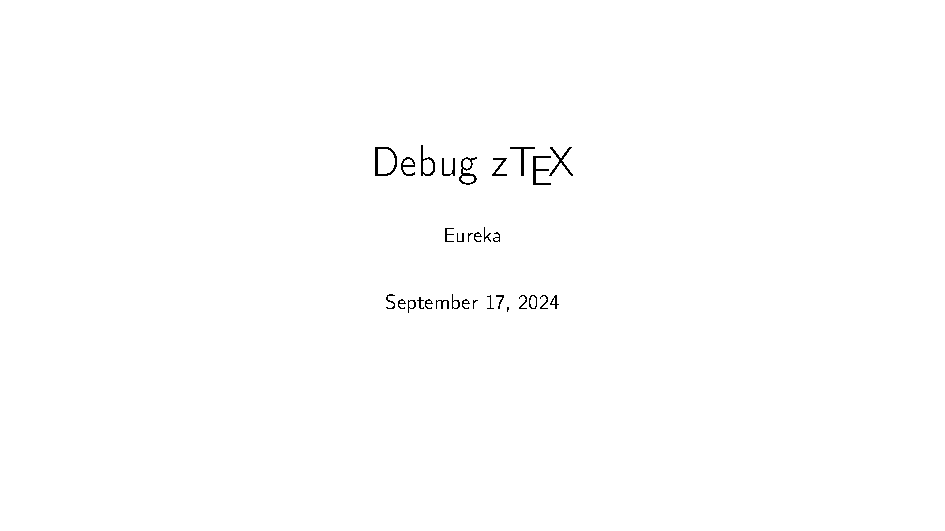
\includepdf[frame, nup=3x5, pages=-, delta=8 8]{zslide_example.pdf}

Hello world 

\newpage

WORLD
\end{document}



\documentclass[tikz]{standalone}
\usepackage{tikz}
\usepackage{tikz-qtree}
\usetikzlibrary{shapes, trees,calc,positioning, arrows.meta}
\definecolor{Red}{HTML}{e32b2d}
\definecolor{Green}{HTML}{15821b}
\definecolor{Blue}{HTML}{0984e3}
\def\deft#1{\texttt{\textcolor{Blue}{#1}}}


\begin{document}
\begin{tikzpicture}[
    >=Latex,
    level distance=65,
    edge from parent/.style={draw, edge from parent fork down},
    frontier/.style={distance from root=360},
    normalKey/.style={draw, rectangle, rounded corners, fill=gray!25},
    boolKey/.style={draw, rectangle, rounded corners, fill=Red, text=white},
    metaKey/.style={draw, rectangle, rounded corners, fill=Green, text=white},
  ]
  \Tree
    [.\node[normalKey] {z\LaTeX{} Options};
      [.\node[boolKey] {hyper}; \deft{false} ]
      [.\node[boolKey] {fancy}; \deft{false} ]
      [.\node[normalKey] {lang}; 
        [.\node[normalKey, fill=Blue] {en}; ]
        [.\node[normalKey] {cn}; ]
      ]
      [[.\node[normalKey] {class}; 
        [.\node[normalKey, fill=Blue] (articleL) {article};  ]
        [.\node[normalKey] {book};     ]
        [.\node[normalKey] (ctexbookR) {ctexbook}; ]
      ]]
      [.\node[normalKey] (classOptionC) {classOption};]
      [[.\node[metaKey] {packageOption};] ]
      [[[[.\node[metaKey] {layout}; 
        [.\node[boolKey]   {margin}; ]
        [.\node[boolKey]   {slide};  ]
        [.\node[normalKey] {aspect}; ]
      ]]]]
      [[[.\node[metaKey] {section};]] ]
      [.\node[metaKey] {toc};
        [.\node[normalKey] {column}; ]
        [.\node[normalKey] {title}; ]
        [.\node[normalKey] {title-vspace}; ]
      ]
      [.\node[metaKey] {mathSpec};
        [.\node[normalKey] {envStyle}; 
            [.\node[normalKey, fill=Blue] {plain}; ]
            [.\node[normalKey] {leftbar};    ]
            [.\node[normalKey] (annotateC) {background}; ]
            [.\node[normalKey] {fancy};      ]
            [.\node[normalKey] {shadow};     ]
            [.\node[normalKey] {paris};      ]
        ]
        [[.\node[normalKey] {font}; 
          [.\node[normalKey] {newtx}; ]
          [.\node[normalKey] {mtpro2}; ]
          [.\node[normalKey] {euler}; ]
          [.\node[normalKey] {mathpazo}; ]
          [.\node[normalKey, fill=Blue] {Computer Modern}; ]
        ]]
        [.\node[boolKey] {alias}; \deft{false} ]
      ]
      [[.\node[metaKey] {bib\_index}; 
        [.\node[boolKey] {load}; \deft{false} ]
        [.\node[normalKey] {backend}; ]
        [.\node[normalKey] {source}; ]
      ]]
      [.\node[metaKey] {font}; 
        [.\node[boolKey] {config}; \deft{false} ]
      ]
    ]
  % lines
  \draw (articleL.south) |- ++(0, -1.5em) -| (ctexbookR.south);
  \draw ($(articleL.south)+(3em, -2.5em)$)node[draw, rectangle, below] {Valid Options} -- ++(0, 1em);
  \draw[->, dashed] ($(articleL.south)+(6.4em, -3.3em)$) -| (classOptionC);
  % annotatations
  \node[text=Blue, rectangle, draw] at ($(annotateC)+(0, -8em)$)  {\texttt{default Value}};
  \node[boolKey] at ($(annotateC)+(0, -10em)$)  {Bool Value};
  \node[metaKey] at ($(annotateC)+(0, -12em)$)  {Meta Key};
  \node[metaKey, fill=Blue, text=black] at ($(annotateC)+(0, -14em)$)  {default Value};
  \draw ($(annotateC)+(-5em, -16em)$) rectangle ++(10em, 10em)node[right=-5em, above] {\textbf{Mind Map Legends}};
\end{tikzpicture}
\end{document}









\documentclass{article}
\usepackage{graphicx}
\usepackage{geometry}
\usepackage{xcolor}
\usepackage{minted}
\definecolor{bg}{rgb}{0.95,0.95,0.95}
\setminted{
  fontsize=\small,
  % bgcolor=bg, 
  breaklines=true, 
  tabsize=2,
  breakanywhere=true,
  breaksymbolright=$\swarrow$,
  breakanywheresymbolpre=$\swarrow$,
  breaksymbolleft=,
}

\begin{document}
% \newgeometry{hmargin=.5in, vmargin=.75in}
\clearpage
\pdfpagewidth=9in
\pdfpageheight=8in
\newgeometry{top=1in,left=.7in,textwidth=8in,textheight=6in}
\pagestyle{empty}
\AddToHook{shipout/background}{\put(8in, -4in){\makebox(0, 0){{\sffamily\color{gray}\scalebox{5}{\thepage}}}}}
\inputminted{latex}{zlatex.cls}
\end{document}





\documentclass{article}
\usepackage{ztikz}
\ztikzLoadModule{cache}


\begin{document}
\begin{tikzpicture}
  \draw (0, 0) -- (1, 1);
\end{tikzpicture}
\end{document}




\documentclass{article}
\usepackage{ztikz}
\ztikzLoadModule{cache, wolfram}
% \usepackage{xsimverb}


\ExplSyntaxOn
\cs_generate_variant:Nn \xsim_file_write_start:nn {nx}
\NewDocumentEnvironment{NewwolframGraphics}{ O{width=.75\linewidth}m }{
  \newcommand{\mmafile}{#2}
  \xsim_file_write_start:nx {\c_true_bool}{\g__ztikz_mma_path_tl/#2}
  }{ 
  \xsim_file_write_stop:  
  % check if hash changed
  % \ztikz_hash_if_change_cs:x {\g__ztikz_mma_path_tl/\mmafile}   
  % \bool_if:NTF \g__hash_change_bool {
  %   % excute mathematica script
  %   \exp_args:Nx \sys_shell_now:n {wolframscript~ -script~ \g__ztikz_mma_path_tl/\mmafile} 
  %   \includegraphics[#1]{\g__ztikz_mma_path_tl/\mmafile.pdf}
  %   \typeout{Writing~ 'mmafig'~environment~source~to~\tl_use:N \g__ztikz_mma_path_tl/\mmafile}
  % }{
  %   \includegraphics[#1]{\g__ztikz_mma_path_tl/\mmafile.pdf}
  %   \typeout{skip~recompile~by~wolframscript,~using~the~cache~picture~\int_use:N \g__mma_picture_index_int}
  % }
  % % step picture index
  % \int_gadd:Nn \g__mma_picture_index_int {1} 
}



% raw test
% \xsim_file_write_start:nx {\c_true_bool}{\g__ztikz_mma_path_tl/example_3.wls}
% HELLO-WORLD
% \xsim_file_write_stop: 
\ExplSyntaxOff

\begin{document}
\begin{NewwolframGraphics}[width=.75\linewidth]{example_3.wls}
figure = NumberLinePlot[
    {Interval[{5, Infinity}], Interval[{2, 7}]}, 
    AxesStyle->Arrowheads[{0, 0.03}]
];
Export["./ztikz_output/mma_data/example_3.wls.pdf", figure];
\end{NewwolframGraphics}




% \wolfram{Series[Exp[x], {x, 0, 5}]}

% \(\wolframResult\)

% \[\wolframResult\]
\end{document}






\documentclass[
  hyper,
  fancy,
  lang=en,
  class=book,
  layout={margin=true, slide, aspect=16|9},
  classOption={11pt, oneside, leqno},
  mathSpec={envStyle=paris, font=euler}
]{zlatex}
\zlatexColorSetup{
  link     = red,
  theorem  = blue
}


\title{l3build-Test}
\author{Eureka}
\date{DATE}
\begin{document}
\maketitle
\frontmatter
\tableofcontents
\newpage
\mainmatter
\chapter{FISRT}
\section{Layout Test}
A 

\begin{figure}
  \includegraphics[width=.5\linewidth]{example-image-a}
  \caption{Margin-Fig}
	\label{fig:Margin-Fig}
\end{figure}


\section{Hyperref Test}
THM-\cref{thm:pythagorean}.FIG-\ref{fig:Margin-Fig}


\section{Class Options Test}
\centerline{\zlatexOptions}


\section{Math Env and Font Test}
\begin{theorem}[pythagorean theorem]\label{thm:pythagorean}
Right-Triangle
\begin{align}
  & a^2 + b^2 = c^2 \\
  & \mathrm{a} = b
\end{align}
\end{theorem}
\end{document}